Como culminación del trabajo realizado durante los últimos cuatro meses, se integró 
finalmente el bloque de la fuente \textit{buck} con el bloque de la LDO 
(ver Fig.~\ref{fig:ldo+buck}). 

\begin{figure}[H]
    \centering
    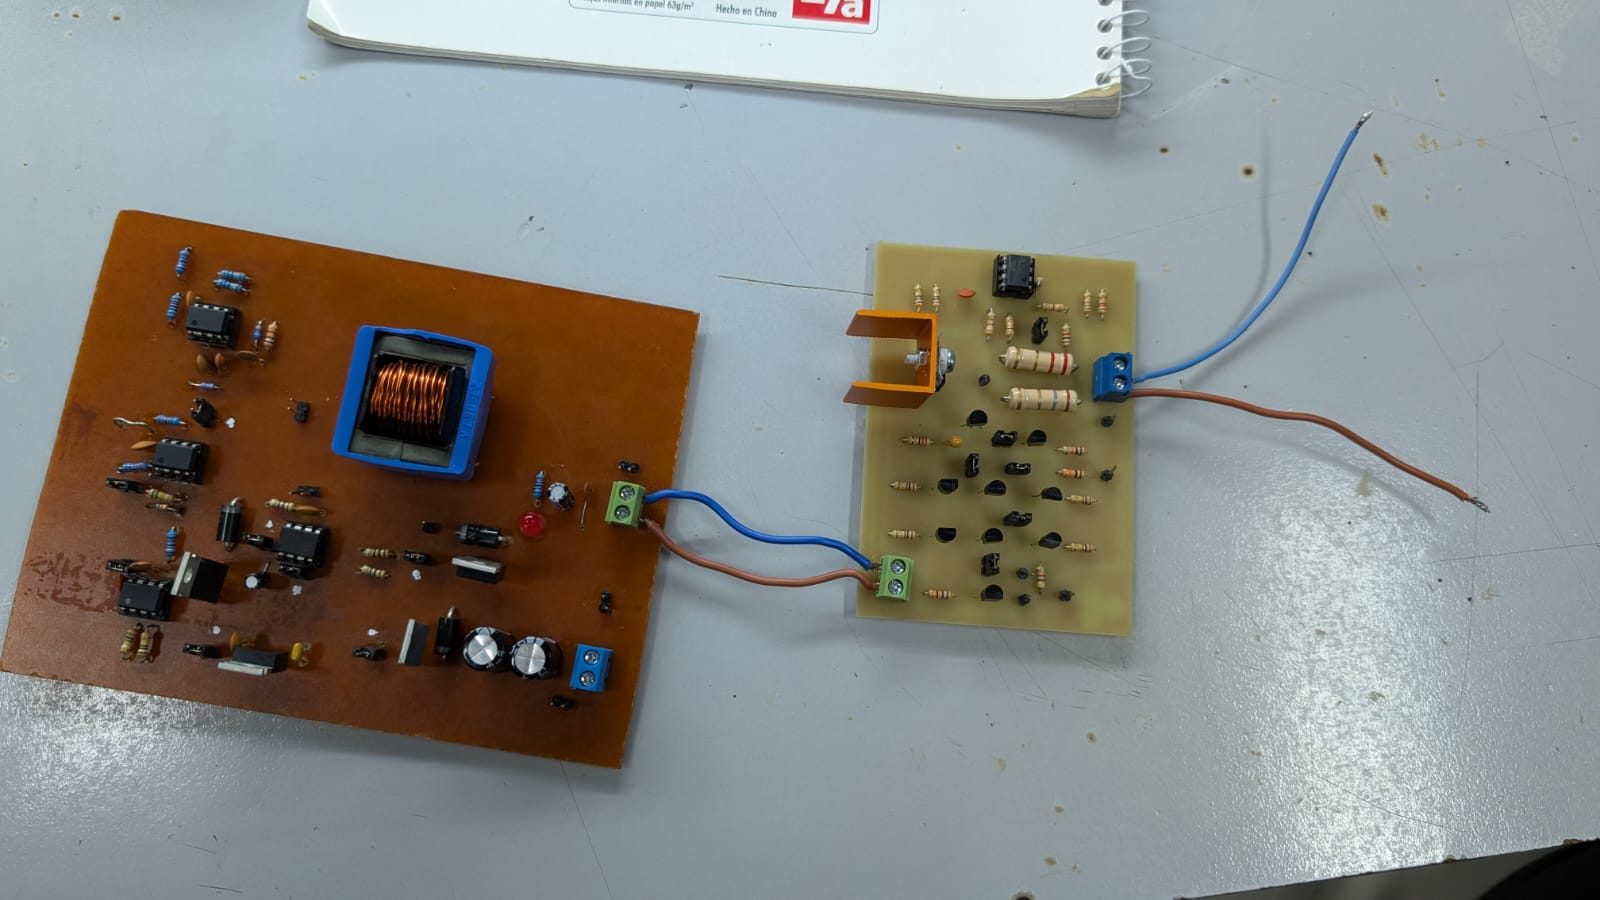
\includegraphics[width=0.65\textwidth]{img/ldo+buck.jpeg}
    \caption{Imagen de la integración de los dos bloques.}
    \label{fig:ldo+buck}
\end{figure}

A partir de esta prueba se verificó el funcionamiento completo del sistema. En 
particular, se observó que la salida de la LDO se mantiene efectivamente 
en \(\SI{5}{\volt}\) para distintos valores de resistencia de carga.

Además, al disminuir la resistencia de carga por debajo de 
\(\SI{3.33}{\ohm}\), se comprobó que se activa correctamente el mecanismo de 
\textit{foldback}, limitando la corriente y reduciendo la tensión de salida. 
Esto confirma que tanto la regulación como la protección de la fuente funcionan 
de acuerdo con lo esperado.

En conclusión, se cumplen con las especificaciones de diseño.

